\section{Results}
\label{sec:results}

The primary experiment is the Class~A search for a drifting, unresolved
spectral carrier: \NWinA{} fine-channel windows toward \NSysClassA{}
systems, \EdrNWinA{} of which are channelised finely enough on the criterion
of \S\ref{sec:statistic} to tell a drifting carrier from a stationary one.
The Class~B search for an unresolved spectral excess is secondary
and carries no drift discrimination: \NWinB{} coarse windows. Together they
are the \NWindows{} windows of the primary census. \textbf{No event
satisfied the confirmation criterion set out in \S\ref{sec:summary}.} What
follows is first how deep the search reaches, and then what it found and how
each finding was disposed of.

\subsection{Sensitivity: the power at which a carrier would have crossed
the threshold} \label{sec:pninetysel}

\emph{The median system, on its best window, would have produced a threshold
crossing from a carrier of $\EirpNinetySysMedA$\,W.} Across the \NSysClassA{} systems those limits
run from $\EirpNinetySysLoA$ to $\EirpNinetySysHiA$\,W
(Fig.~\ref{fig:classasens}a), and \NSysEfifteen{} of the systems reach
$10^{15}$\,W. The median Class~A \emph{window} reaches
$\EirpNinetyWinMedA$\,W.
Over the \EdrNWinA{} windows in which the searched drift crosses a channel
(\S\ref{sec:statistic}) the search covers \EdrUnionGHz\,GHz toward
\EdrNSys{} systems, and their median system limit is \ScEdrMedPct{} per cent
\ScEdrMedSense{} than the figure above.

\emph{They are a recovery completeness of one epoch, and not a threshold.}
Artificial carriers were injected at a random sub-channel phase and a random
drift from each window's own grid, then recovered through the unchanged
pipeline; the power at which nine in ten come back is
$\mathrm{EIRP}_{90}$, the only sensitivity quoted here. It is measured
through the single-epoch trigger and the localisation at the stellar position
inside one execution block. \textbf{It is therefore the power at which a
carrier would have produced a crossing and not the power at which one would
have been confirmed}, because confirmation needs a second and separated epoch, which the archive
supplies for some systems and not others (\S\ref{sec:confirmability}). The \NCtrl-position spatial rank
decides nothing and is not charged against it either: charging it would cost
a further factor $\SensCostLike$, and in \SensNRingHiUnres{} bright-ring
windows it could not be met at any injected power (Fig.~\ref{fig:strata}).

\emph{Measured that way the completeness is one number for the class.} Nine
carriers in ten are recovered at $\EirpNinetyMultA\,P_{\rm trig}$, and the
sampling error of that pooled value is $\pm\SensBootPct$ per cent -- a
statement about the class average and about no individual window. It is a
total power set against a nominal threshold, $P_{\rm trig}$ being the bare
$\LtCommonSnr\sigma$ of the window itself. The loss a channel-confined
carrier suffers to the correlator's spectral response is carried by the
injected tones, so it sits inside the measured factor -- $\times\RpRespFac$
of it -- and is not applied to the result as well
(Appendix~\ref{app:conventions}). Every one of the \SensNInj{} directly
injected Class~A windows resolves a ninety per cent point of its own, and the
value does not depend on the brightness of its control ring: the
\SensNRingHi{} windows whose ring carries resolved emission come back at
$\SensRingHi\,P_{\rm trig}$ against $\SensRingLo$ for the rest
(Fig.~\ref{fig:strata}). Class~B carries its own factor $\EirpNinetyMultB\,P_{\rm trig}$, which
sets the limits for Barnard's Star, Wolf~359 and Proxima. It is measured the
same way, from \SensNToneCoarse{} carriers injected into \SensNInjCoarse{}
coarse windows of \SensNInjCoarseBlock{} execution blocks.

The calibration of that factor is good to
$\times\SensFacLo$--$\times\SensFacHi$ (Table~\ref{tab:p90budget}), which is
an interval on the median and on the counts and not on any one window's
limit. The median system's limit above carries it -- $\TfMedCalLo$ to
$\TfMedCalHi$\,W -- so the second figure of that median is set by the
calibration rather than by the depth of any observation.

\emph{Every limit quoted here is nominal in one respect: it excludes
atmospheric decorrelation.} An injected carrier is added to already
calibrated visibilities and so suffers none, whereas a real carrier does, and
the bias runs one way only. Measured block by block from the phase rms the
observatory records on each block's phase calibrator
\citep[\S\S10.4.11, 11.3.1]{ALMAHandbook}, through the standard phase-scatter
relation \citep[Eq.~3]{Richards2022}, it leaves the median limit optimistic
by \SensDecorPct{} per cent. It is least secure at the top of the frequency
range: \SensDecorHiPct{} per cent for the median window above
\SensDecorHiGHz\,GHz, and \NmDecHiPct{} per cent at the ninetieth percentile
of windows. Across the systems' own best windows -- the limits a reader uses
-- the median is \NmDecSysMedPct{} per cent, and \NmDecNBigSys{} of them
carry more than a tenth: \NmDecBigSys. The strongest limits are among the
least affected. Of the ten deepest limits in the survey only
\NmDecDeepBigSys{} carries more than a twentieth, at \NmDecDeepBigPct{} per
cent, and \NmDecNoRecSys{} carries no estimate at all, its delivery exposing
neither a phase record nor a baseline to match on.
That best window lies in a block with no phase record of its own for
\NgNDecImpSys{} of the \NSysClassA{} systems, so the figure beside it in
Table~\ref{tab:persys} is imputed from the blocks matched to it in baseline
and starred there, against \NgNDecMeasSys{} measured. The deepest limits are
no better served than the rest: of the \NgNDeep{} deepest, \NgNDeepMeas{}
carry a measured correction and \NgNDeepImp{} an imputed one. The median
above is therefore a mixture of the two, \NgDecMeasMedPct{} per cent over the
measured and \NgDecImpMedPct{} over the imputed.

\textbf{The \RpDecNUn{} blocks whose delivery exposes no such record are not
a random subset of the \SensDecorNBlkTot}: of the \NbDecNUnBl{} of them that
carry a baseline, \NbDecPctTwelveUn{} per cent were taken with the 12\,m
array, against \NbDecPctTwelveMeas{} per cent of the blocks that do expose a
record, and it is that array's long baselines that lose coherence.
Within each array the two sets are not distinguishable --
\NbDecBlSevenUn{} against \NbDecBlSevenMeas\,m in the median on the compact
array and \NbDecBlTwelveUn{} against \NbDecBlTwelveMeas\,m on the 12\,m one
-- so what the archive withholds is a configuration rather than a baseline.
Matching each of their windows
to the measured blocks within a factor of two in baseline length puts the
correction at \RpDecMatchMed{} per cent in the median, rising to
\RpDecMatchHi{} per cent were their coherence as poor as the ninetieth
percentile of the blocks matched to them, so their limits are conditional on
a calibration performance the archive does not report. \emph{That is why this
term is stated and not folded in}: the three factors that are applied are
available for every window of the census, while this one is available for
\SensDecorNBlk{} blocks of \SensDecorNBlkTot{} and the rest are measurably
the harder ones. Folding it in where it is known would leave a set of limits
that is neither corrected nor uncorrected.

\emph{Three further factors act window by window, and all three are divided
out of the limits above rather than quoted beside them}
(Appendix~\ref{app:conventions}). The first is the primary-beam response
$A$ at the star's own offset from the pointing centre, which is what turns a
measured noise into a flux at the star. It divides into the limit, so its
cost is the factor $1/A$: nothing in the median window, where the star is all
but on axis, more than $\times2$ in \NmBeamNFacTwo{} windows and
$\times\NmBeamFacWorst$ in the worst. It is evaluated on the full width the
observatory documents, at each window's own dish diameter and centre
frequency. Of the two widths available that is the one that follows a blocked
circular aperture (Appendix~\ref{app:conventions}). Only the
\BmNAboveTenPct{} windows furthest off axis, toward \BnStarList, would move
by more than a tenth on the wider of the two, where they would be up to
\BmShiftMaxPct{} per cent deeper. One of those windows is its own system's
best: \BnBestSys{} is corrected by $\times\BnBestFac$ at that window's
response of \BnBestResp, and that limit carries the beam-model departure as a
systematic beside the calibration interval.

The second is the annual parallax, which the search's phase centre omits. It
displaces the star by at most \SensBeamsMax{} of a synthesised beam and makes
the median Class~A limit shallower by \PxaShiftWinPct{} per cent, while
\PxaNMissing{} windows in \PxaNMissingEb{} blocks, toward
\PxaMissingStars, have no astrometric keys and are left uncorrected.
\PxaNMissingTop{} of those are \PxaMissingTopStar's, where the displacement
follows from the catalogued parallax instead and leaves the tabulated limit
optimistic by at most \BmEpsPxBoundPct{} per cent
(Appendix~\ref{app:pbresp}). That correction is concentrated rather than general, which is
why the median limit moves far more than the median window's own factor
(Table~\ref{tab:p90budget}): \RpPxNNone{} of the \NWinA{} windows need none
at all, while \RpPxNBig{} lose more than a tenth and lie around the middle of
the distribution of limits.

The third the injections do not reproduce at all, each carrier being laid
down at one frequency per integration while a real one sweeps within it. What
the sweep costs is the mean of the delivered channel response over it, these
channels being wide enough that a sweep moves a carrier's dwell time between
channels rather than destroying coherence inside one
(Appendix~\ref{app:conventions}). \textbf{It costs nothing in the median
window and up to $\times\SmcFacWorst$ in the \SmcNAbove{} finest-channel
ones, which are also the deepest}, and it takes the best Class~A window from
$\SmcWinLoWas$ to $\EirpNinetyWinLoA$\,W.

\emph{The net bias on one window's limit is therefore of either sign.} The
decorrelation leaves a limit optimistic, while the injected profile falls
\InjShortPct{} per cent short of the exact channel response and leaves it
conservative by that much (Table~\ref{tab:p90budget}). In the median window
the second is the larger, so the quoted limit is conservative by
\NmNetConsPct{} per cent; at the ninetieth percentile of the systems' own
best windows the first is, and the quoted limit is optimistic by
\NmNetOptPct{} per cent, rising to \NmNetOptMaxPct{} per cent for the most
affected system. Neither direction describes the sample, and Table
\ref{tab:persys} gives the decorrelation system by system so that a reader
can apply it to the one limit in question.

\emph{Carriers were injected directly into \SensNInj{} of the \NWinA{}
Class~A windows, \SensNInjPct{} per cent, and the result transferred to the
remaining \SensNTransfer. That transfer is the dominant caveat on everything
above.} The injected windows are the Class~A windows of execution blocks
drawn in a random order, balanced by band and array; they hold
\SensNCrossAch{} crossings against the \SensNCrossExp{} the population rate
predicts. \emph{The unit is the block and not the window}, because a block's
calibrated visibilities are what an injection campaign has to rebuild, so
band and array were fixed by the draw and the conditions that vary within a
block were compared with the population afterwards.

\textbf{That comparison covers \RpNAxis{} properties} -- channel width,
integration time, noise, control-ring brightness, the channels a carrier at
the drift ceiling crosses in one track, and the intra-integration retention
-- and on every one the injected windows span the central eight-tenths of the
population, five of them agreeing in the median to \RpCovOtherPct{} per cent.
The sixth, \RpCovWorstAxis, does not: the injected windows are
$\times\RpCovWorstRatio$ noisier, which follows from drawing whole blocks. It
is also the property the measurement is built to be insensitive to, each
ladder being in units of its own window's threshold, and that insensitivity
is measured rather than assumed -- splitting the injected set at the median
of each property in turn moves the ninety per cent point by at most
\RpFacShiftMax\,$P_{\rm trig}$. The injected set also spans both delivered
response forms, \TfInjNat{} windows at the native channelisation and
\TfInjAvg{} with channels averaged online, and splitting it there moves the
point by \TfFacShift\,$P_{\rm trig}$. The draw controlled the array, but the
achieved mix still departs from the population by \SensCovWorstPct{} per cent
of the sample; re-weighting the pooled curve by the survey's own composition
gives $\SensPooledArrWeighted\,P_{\rm trig}$ against the adopted
$\EirpNinetyMultA$.

\textbf{A window that was not injected therefore carries an estimated
$\mathrm{EIRP}_{90}$.} What is carried across is one dimensionless number per
class -- the ninety per cent point in units of the window's own trigger power
-- while the channel width, the noise, the integration time, the primary-beam
response, the parallax displacement and the intra-integration retention that
turn it into a power are each that window's own measurement.
Across the injected windows the ninety per cent point
ranges from $\times\SensIndivFacLo$ to $\times\SensIndivFacHi$ of the
adopted factor, with \NmDispNTenth{} of the \SensNInj{} lying within a tenth
of it. The upper end of that range is one window and not a typical error: the
second largest is $\times\NmDispSecond$. That dispersion, and not the calibration
interval above, is what one uninjected window's own limit is uncertain by.
Two bands and two channelisations of the survey hold no injected window at
all, \NgNExtrapWin{} windows between them, and \NgNExtrapSys{} systems take
their best window from one: \NgExtrapSys. For those the completeness is
transferred across a configuration boundary rather than within one, and the
deepest limit in the survey is among them.
\textbf{The best window was itself injected into for \SmcNMeasSys{} of the
\NSysClassA{} systems}, marked as measured in Table~\ref{tab:persys}; for the
other \SmcNEstSys{} the headline limit is an estimate carrying that
dispersion. Each of the six at its own measured
factor rather than the class average would move by at most \NmOwnDevPct{} per
cent. Over the population the estimate is not biased in a direction one can
name: because a system's limit is its best window, a minimum over several
estimates could favour windows whose own factor falls below the class
average, but drawing each window's factor from the \SensNInj{} measured ones
instead, over \ScRsNTrial{} trials, leaves the per-system median where it
is -- the shift is \ScRsMedShiftPct{} per cent -- and holds the count at
$10^{15}$\,W to \ScRsNLo--\ScRsNHi{} in nine trials in ten.

\emph{A carrier that is not always radiating is penalised in proportion.} The
de-drifted stack runs the length of a whole execution block, so over
\DutyNTrial{} trials at duty cycles down to \DutyCycleMinPct{} per cent the
recovered amplitude followed the duty cycle to \DutyAttenDevPct{} per cent: a
transmitter radiating a tenth of the time needs $\DutyPowFac\times$ the power
quoted above. Those trials carry no drift, so the joint drifting and
intermittent case is not measured here.

\begin{table*}
\centering
\scriptsize
\caption{What sets $\mathrm{EIRP}_{90}$, and in which direction. The
uncertainty on the calibration is an uncertainty on the class-average factor,
and so on any statistic formed over many windows; its flux term is
band-dependent, so the submillimetre windows carry the larger combined
figure. The spread between windows
is an observed dispersion and is the statement about one window's own limit;
the signed terms are biases, stated with their direction rather than folded
into an error bar, and the decorrelation term is measured in \SensDecorNBlk{}
of the \SensDecorNBlkTot{} blocks and not imputed to the rest.}
\label{tab:p90budget}
\setlength{\tabcolsep}{2pt}
% GENERATED by sens_r11.py -- do not hand-edit.
\begin{tabular}{@{}l@{~~}r@{~~}>{\raggedright\arraybackslash}p{0.61\linewidth}@{}}
\hline
 & value & what it does to the limit \\
\hline
Class-average completeness & $\times3.03$ & nine carriers in ten recovered at this multiple of a window's own trigger power. \emph{Measured} in the 49 Class~A windows injected directly and \emph{estimated}, at this factor, in the other 356 \\
\hline
\multicolumn{3}{@{}l}{\emph{Uncertainty on that calibration} (per cent), combined in quadrature} \\
The factor itself & $\pm2$ & sampling error of the pooled value over the 49 injected windows \\
Absolute flux scale & $\pm\BudFlux$ & the observatory's own band-dependent specification (\BudFluxSource): \BudFluxSpec, weighted over this sample's bands \\
Distance and visibility scale & $\pm\BudDistVis$ & the Gaia parallaxes, which enter as $d^{2}$, and the block-to-block visibility scale \\
\emph{Combined} & $-11/+11$ & $\times0.89$--$\times1.11$ on the factor, and so on the median limit and on the system counts; $\pm\BudCombWorst$ for the \BudNHiWin{} Class~A windows in \BudHiBandWord~\BudHiBands, at \BudHiGHzList\,GHz \\
\hline
\multicolumn{3}{@{}l}{\emph{Spread between windows}. An observed dispersion, not an error bar.} \\
Window to window & $\times0.80$--$\times1.58$ & the 49 injected windows resolve 2.41--4.80\,$P_{\rm trig}$ individually, \NmDispNTenth{} of them within a tenth of the pooled value and the second largest at $\times\NmDispSecond$. This, and not the interval above, is what an estimated limit is uncertain by; it is wider, and it applies to \SmcNEstSys{} of the \NSysClassA{} systems \\
\hline
\multicolumn{3}{@{}l}{\emph{Applied}. Folded into every limit quoted, and so not combined with the above.} \\
Intra-integration smearing & $\times1.00$--$\times\SmcFacWorst$ & a carrier sweeps through part of a channel within one integration and the injected ones do not: $\eta_{\rm smear}$ at the drift that sets a ninety per cent point, from each window's own integration length where it is recorded (\SmcNMeas{} windows) and from the longest delivered anywhere where it is not (\SmcNBound) \\
Primary beam & $\times1.00$--$\times\NmBeamFacWorst$ & the star is not at the pointing centre, so each limit is divided by the response at its own offset, on the full width the observatory documents. Nothing in the median window; the \BmNAboveTenPct{} windows furthest off-axis carry the departure of that form from a blocked circular aperture, up to \BmModelMaxPct{} per cent, as a one-sided systematic \\
Annual parallax & $\times1.00$--$\times2.06$ & the phase centre omits it, so each limit is divided by the amplitude a compact source retains at its own displacement, a median \PxaLossMedPct\,per cent \\
\hline
\multicolumn{3}{@{}l}{\emph{Signed terms}. A bias is not an error bar and is not added to one.} \\
Channel response & $\times\RpRespFac$ & the share of a channel-confined carrier the peak channel keeps. Carried by the injections, so already inside the completeness above, which is this factor times a margin of $\times\RpMarginNinety$ over the nominal trigger \\
\quad its residual & $+\InjShortPct$ & the injected profile falls short of the exact response: \emph{conservative} \\
Decorrelation & $+0/+\SensDecorPct$ & measured block by block from the phase rms the observatory records on each block's phase calibrator, which an injected carrier does not suffer and a real one does: $+\SensDecorHiPct$ above \SensDecorHiGHz\,GHz, and more than $+\SensDecorTailLevelPct$ in \SensDecorTailPct{} per cent of windows \\
\hline
\end{tabular}

\end{table*}

\begin{figure}
\centering
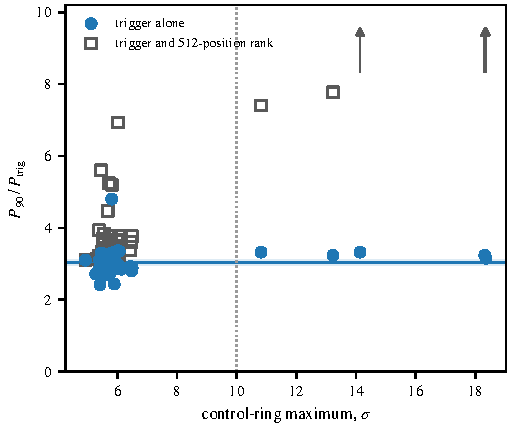
\includegraphics[width=\columnwidth]{figures/sens_ring.pdf}
\caption{Why one completeness factor serves the whole class. Each of the
\SensNInj{} of the \NWinA{} Class~A windows injected directly is plotted at
the power that recovers nine carriers in ten, against the maximum of its own
\NCtrl-position control ring. Filled circles are the criterion adopted
here -- the trigger and localisation at the star -- with the pooled value
and its uncertainty as the line and band; they show no trend with the ring.
Open squares add the demand that the carrier outrank every control position,
and arrows mark the windows that then reach ninety per cent at no injected
power. Dotted, the $\SensRingRule\sigma$ ring brightness above which a ring
carries resolved emission rather than noise.}
\label{fig:strata}
\end{figure}

\begin{figure*}
\centering
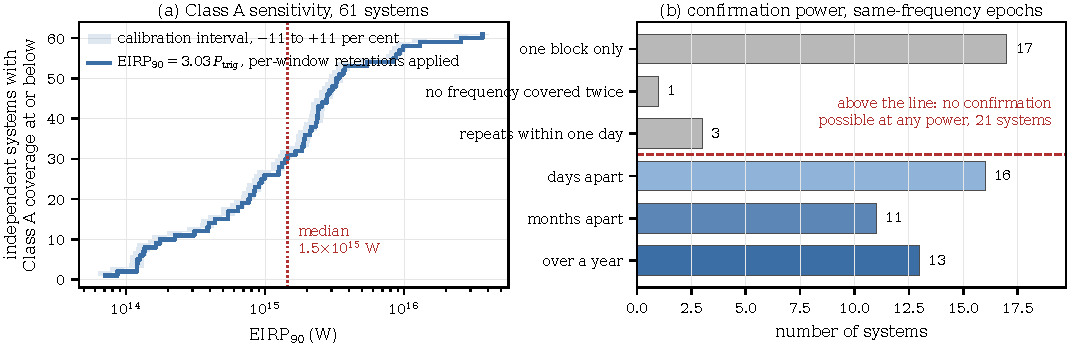
\includegraphics[width=\textwidth]{figures/classa_sensitivity.pdf}
\caption{\textbf{The two completenesses of the carrier search, over the same
\NSysClassA{} systems.} \emph{(a)}~Single-epoch trigger completeness: the
cumulative number of systems whose best window reaches a given
$\mathrm{EIRP}_{90}$ (Table~\ref{tab:quantities}), evaluated as
$\EirpNinetyMultA\,P_{\rm trig}$ with each window's own primary-beam,
annual-parallax and smearing retentions applied and atmospheric
decorrelation excluded, which Table~\ref{tab:persys} gives system by system;
the shaded band is the calibration interval of
Table~\ref{tab:p90budget}. \emph{(b)}~Confirmation completeness, for a
carrier whose stellar-frame frequency at the two epochs agrees to within half
a native channel, which no
amount of power buys: systems grouped by the longest separation between two
execution blocks of different observing sessions covering a common
frequency, which is what the criterion of \S\ref{sec:summary} requires,
over the primary census together with every repeat block the recurrence
test of \S\ref{sec:etacrv} reads. \textbf{Left of the dashed line,
\ZcNoRepSys{} systems have no such pair, and for them confirmation was not
possible at any sensitivity in panel~(a)}. The two panels are separate
statements and neither follows from the other: (a) is the power at which a
carrier crosses the trigger in one block, (b) whether a crossing there could
then have been tested at all.}
\label{fig:classasens}
\end{figure*}

\subsection{The nearest stars: Barnard's Star and Wolf~359}
\label{sec:barnardswolf}

Barnard's Star is the second-nearest stellar system and Wolf~359 the third if
brown dwarfs are excluded, and to our knowledge these are the first millimetre
or submillimetre technosignature limits for either; earlier radio searches of
the nearest stars have worked at centimetre wavelengths \citep{Enriquez2017,
Price2020, Margot2023}. Both are non-detections. \emph{Both limits come from
the secondary Class~B experiment and not from the carrier search}: the archive
holds only coarse Band~6 windows toward these stars, so what is constrained is
an unresolved spectral excess and not a drifting carrier. On the $\mathrm{EIRP}_{90}$ convention of \S\ref{sec:pninetysel}
Barnard's Star reaches $\EirpNinetyBarnLo$--$\EirpNinetyBarnHi$\,W over
\NWinBarn{} windows. Wolf~359 reaches
$\EirpNinetyWolfLo$--$\EirpNinetyWolfHi$\,W over \NWinWolf.

\subsection{Threshold crossings and how each was disposed of}
\label{sec:technosearch}

\emph{The result is a chain of three tests, and it is read in one direction.}
Of the windows the search covers -- the \NWindows{} of the primary census
and the archival-tail blocks beside them -- \EvNCrossRaw{} hold a cell
reaching $T\geq5$ at the stellar position. \EvNCrossFlag{} lie in the one
execution block that fails the quality criterion of \S\ref{sec:bdblock}, which
was written after the condition was seen in that block and is insensitive to
where the line was drawn (Appendix~\ref{sec:blockquality}), so the population
that characterises the search is the \EvNCrossQp{} in quality-passing data and
those \EvNCrossFlag{} are reported beside it. The molecular-line mask is $\pm\MaskHalfKms$\,km\,s$^{-1}$ wide in each
star's own rest frame, and it places \MkNCoinc{} of the \EvNCrossQp{} within
that distance of a catalogued transition. Of those coincidences, \MkNSODecideWord{} are with a species no debris disc
has been shown to carry, and are reported rather than acted on
(Appendix~\ref{app:linemask}). That leaves
\EvNAttrQp{} crossings attributed and \EvNUnattrQp{} unattributed. The attributions are kinematic and not an accident of bandwidth: in the
frame the correlator delivered, the crossings with a measured peak frequency
crowd onto the transitions these setups were tuned to far more tightly than a
free landing on their own grids would put them (Appendix~\ref{app:rfi}). Of the unattributed,
\EvNRankQp{} outrank all \NCtrl{} control positions of their own window, and
none was found again in any other epoch covering its frequency. \textbf{No
crossing survives the chain, and this survey reports no detection.}
Figure~\ref{fig:chain} counts what survives each step and the crossing
ledger lists every crossing, a sample of it in Table~\ref{tab:ledger}.

\emph{Anything bright in a window hides a weaker carrier behind it, so the
weaker cells were sought too.} The de-drifted statistic is retained in every
channel, so behind a window's tabulated crossing -- its largest cell --
weaker above-trigger cells can be read as well, neighbouring channels counting
as one. \CkNWin{} of the \NWinA{} Class~A windows retain such a profile and the
other \CkNWinNotCov{} retain none. Re-read that way they hold \CkNPrimary{}
maxima at or above the trigger -- one for each of the census's
\CkNCrossCenA{} Class~A crossings but \CkMissStar's, whose own window retains
no spectrum -- and \CkNSecondaryWord{} weaker cells besides, in \CkNSecWin{}
windows and as many as \CkNSecMax{} in one. \CkNSecAttr{} of the weaker cells
are the resolved carbon monoxide of a disc spread over channels. The
\CkNSecUnattrWord{} unattributed ones, toward \CkSecStars, each have
\CkCovLo--\CkCovHi{} covering blocks, and \CkNRecurWord{} reaches the trigger
in any of them: the deepest repeat is $T_\star=\CkTrepHi$. Applied to the window maxima the rule returns \CkRegN{} of the
\EvNCrossRaw{} tabulated crossings to \CkRegDev{} of a channel. The
\CkRegMiss{} it misses are the \EvNCrossFlag{} of the failing block, whose
repaired profile was not retained, and crossings whose own window retains no
usable profile.
Cells are counted in the controls too, and outside the mask the star holds
\CkRatioLo--\CkRatioHi{} times as many as a control position at every level
from $T=\CkLadderLo$ to the trigger, with no step where a carrier search would
put one; the expectation that follows is \S\ref{sec:trigunif}'s.

\subsubsection{The unattributed count is what the control positions predict}
\label{sec:trigunif}

The trigger is a threshold on a statistic and not a false-alarm rate: the
number of searched channel\,$\times$\,drift cells per window spans
\TuCellsDecades{} decades, so one level buys very unequal protection. How
many crossings chance should produce is therefore measured window by window,
over the \CeNWin{} Class~A windows of the census and with one condition on
both sides of the comparison: a cell at the stellar position that reaches the
trigger and that the line mask does not attribute. A window's own \NCtrl{} control positions measure how often a position in
that field reaches the trigger, and the channels their exceedances land on
measure how often one of them would be attributed. Both are read from the
data themselves, and Appendix~\ref{app:falsealarm} gives that accounting. The control positions differ from the star in one respect that
bears on this: they carry no continuum, so a calibration error that varied
with frequency would raise the star and not them. Measured on the continuum
these stars are found to have, in its own block, no window in the survey
could reach the trigger that way: the least demanding would need
\CyEpsMinPct{} per cent (Appendix~\ref{app:radius}); and the mild stellar
excess of
\S\ref{sec:technosearch} does not follow that continuum as such an error
would, standing at \CkRatioContBright{} in the brightest third of the
\CkNContWin{} windows whose star has a photospheric estimate against
\CkRatioContFaint{} in the faintest. These fields' own control positions predict \CeExp{} unattributed
Class~A crossings and \CeObs{} are found. A count that large or larger arises
by chance with probability \CeProbNull. That sum over the control positions
is the expectation adopted here. The stars do carry \CeStepPct{} per cent
more above-threshold cells than their own controls below the trigger, and
that excess has no identified cause; the rate adopted is the control
positions' own, which is the smaller of the two and the more demanding of
the count under test. Carried in as a sensitivity test the excess would give
\CeExpX{} and a probability of \CeProbStep.
Counting cells rather than windows on both sides moves the two
together, so nothing turns on either choice (Appendix~\ref{app:falsealarm}). A further \CeNTailCrossWord{} unattributed
crossings, both toward \CeTailStar, lie in archival-tail blocks the catalogue
does not tabulate window by window, and enter neither side.

What that establishes is consistency with the expectation these fields' own
control positions set, under the assumptions above, and not that the
unattributed crossings are noise: the most this comparison could not have
rejected is \CeAddLim{} further crossings against those same control
positions, which is a bound on compatibility and not a confidence limit on a
population of transmitters (Appendix~\ref{app:falsealarm}). What tests each
crossing individually is the recurrence test of \S\ref{sec:etacrv}.

\subsubsection{One execution block accounts for four of the crossings}
\label{sec:bdblock}

\BdNCross{} crossings belong to \BdStar{} (\BdAlias), all of them in one
ACA execution block, \texttt{\BdBlock}, whose whole field is above threshold.
\BdNCtrlAbove{} of its \BdNCtrl{} control positions exceed $T=5$, where the
median of a window's own control ensemble is \BdSurvCtrlMed{} across the
survey. Its single-integration noise is as predicted, \BdRmsMeas\,Jy against
\BdRmsPred\,Jy, but it does not integrate down. A jackknife on the channel
mean gives \BdJack\,Jy against \BdThermal\,Jy thermal, \BdJackRatio{} times
too large, while neighbouring channels stay uncorrelated (\BdChanCorr). What the two numbers describe is a
residual that persists from one integration to the next and differs from
channel to channel. Equation~\ref{eq:tstar} divides by the noise of the
stacked spectrum, which falls as the root of the integration count, so a
residual that does not average down accumulates along a drift track faster
than the denominator grows, and it does so at every position in the field; and
having no part common to the channels of one integration, it is not what the
continuum median of \S\ref{sec:statistic} removes. The \BdNSibling{}
sibling executions of the same field, array and setup reach only
$T_\star=\BdSibTMax{}$ and produce no crossing. \emph{What is inflated is the field and not the star.} The strongest of the
four reaches $T_\star=\EvFlagTStarHi$ where its own controls peak at
\EvFlagCtrlAtHi, and \EvFlagNgeLo--\EvFlagNgeHi{} of the \BdNCtrl{} stand
above the star. The
criterion fails this block and no other, at any threshold between it and the
next most extreme block (Appendix~\ref{sec:blockquality}), so its
\BdNCross{} crossings are reported apart from the \EvNCrossQp{}; Appendix~\ref{app:rfi} carries what the block
might instead be. Milder cases of the same condition are not unique to it:
read window by window the same diagnostic flags \DqNWin{} windows in
\BkFlagNBlock{} blocks, and the \BkFlagNCrossOther{} flagged crossing outside
this block -- \BkFlagOtherStar{} -- is withheld for it too.

\subsubsection{Stellar flares are excluded by a broadband prediction}

The sample contains known flare stars. But a millimetre flare raises every
channel of a window alike, so one able to produce a single-channel crossing at
the trigger must produce a $5\sqrt{N}\sigma$ continuum event in the same
integrations. Over the \FlNCont{} crossings with a recoverable continuum measurement
that prediction runs \FlPredLo--\FlPredHi$\sigma$. The observed continuum
statistic has median \FlObsMed, with $|Z|<3$ in \FlNQuiet{} of them. One block settles it: \FlEgStar{} \texttt{\FlEgEb} holds both a
crossing ($T_\star=\FlEgT$) and the millimetre flare of
\citet{MacGregor2020}, and \emph{that flare contributes \FlEgContrib$\sigma$
to the single-channel statistic} -- raising the continuum at $Z=\FlEgContZ$
while the crossing's own de-drifted track reaches $Z_{\max}=\FlEgTrackZ$.

\subsection{$\beta$~Pictoris: an astrophysical positive control, and the
obstacle it identifies} \label{sec:bpicval}

\emph{A search that finds nothing must show that it could have found
something, and the survey's strongest features show exactly that.} The
pipeline recovers the $\beta$~Pictoris circumstellar carbon monoxide
without being told the disc is there. It recovers it in two
rotational transitions and in \CsBpCoBlocks{} execution
blocks spanning \BpBaselineYr\,yr. Those blocks belong to \CsBpCoSess{}
observing sessions, several of them executions of one session on one
tuning, and each transition is recovered in more than one session: the
closest two sessions to hold the same transition are \CsBpCoSepMinD\,d
apart -- \texttt{\NbSessEbOne} and \texttt{\NbSessEbTwo} in
\NbSessLine{} -- while one session's own blocks here span \QfBpSameSessD\,d
-- so a
repeat between sessions is a repeat between epochs, and a repeat inside one
is not a confirmation however far apart the two blocks fall.
In \NStageOneBpicEb{} of the blocks the star also outranks every control:
\BpicNFlagThree{} Band~3 windows, at $T_\star$ up to \BpicBThreeTsym, and
\BpicNFlagSix{} Band~6 windows at \BpicBSixTsym. The identification is kinematic and does not rest on those
statistics. Carried through the frame chain -- to the barycentre at each
block's own epoch, then to the star's rest frame -- all \BpicPanelNCo{}
crossings lie within \BpicDvCoHi\,km\,s$^{-1}$ of the stellar systemic
velocity, in the two lowest CO transitions of a star with mapped
circumstellar CO \citep{Dent2014,Matra2017}. The Band~3 peaks agree across blocks to
\BpRecThreeTuneChanMax{} channel once each block's own tuning is removed, so
any apparent drift is far below the grid searched. The alternative reading
requires a transmitter placed by coincidence at matched offsets from two CO
transitions of one star.

It is also the control that shows the recurrence test of
\S\ref{sec:etacrv} working in the positive direction: every flagged
$\beta$~Pictoris carbon-monoxide feature is recovered in another execution
block, and each transition in a block of another session as well, the
screened Band~6 window returning
$T_\star=\BpRecTTwo{}$ in the second block of its own recurrence set. A
non-recurrence elsewhere means nothing unless the same machinery recovers a
repeat where one exists.

\emph{One of those blocks is a counterexample, and it is the more useful half
of the control.} In it several of the \NCtrl{} control positions exceed the
stellar statistic, so the spatial rank disfavours a window holding carbon
monoxide known to be real and centred on the star; the disc is resolved on
the scale of the primary beam in that configuration, which is the geometry
the statistic is built to reject. The rank is therefore a test of
compactness and not of authenticity, and on a real extended source it errs
conservatively -- a stronger statement than a clean positive control, because
it bounds the diagnostic's reach as well as demonstrating it
(Fig.~\ref{fig:bpiccontrol}).

%% fig:bpiccontrol MOVED to Appendix B (sections/app_C_spatialnorm.tex),
%% which is the appendix about the spatial statistic this figure bounds.
%% 0.36 pp off the main text; Sec. 5.4 cites it.


HD~48370 is the complementary case and is equally instructive. Its crossing
reaches $T_\star=\HdTsym$, but the control ring rises with the star, to
\HdRingMax, as emission filling the primary beam does. The velocity matches
the prominent CO($2{\to}1$) that \citet{Cataldi2023} report toward the
source and flag as possible cloud contamination. The block's
$^{13}$CO($2{\to}1$) window is bright at the ring and faint at the star.
What identifies the extended emission is therefore the \emph{level} of the
control ring and not the star's rank against it -- the star here outranks
every control -- which is why the window-level flag of
Appendix~\ref{sec:blockquality} is defined on the ring's median.

\emph{Taken together, these two results identify the dominant obstacle for
millimetre technosignature searches, and it is not sensitivity.} The
strongest apparent signals in the quality-passing data are circumstellar and
interstellar molecular emission, the \DqBlockNCross{} highest statistics in the
survey belonging instead to the one block that fails the criterion of
\S\ref{sec:bdblock}: \MkNCoinc{} of all \NCross{} crossings land
on a catalogued transition and \NAttributed{} of them are attributed to it.
The mask that
removes them covers \FrNSpec{} species and costs \MkMaskAPct{} per cent of
the Class~A union bandwidth, and it is nevertheless the single most
productive test in the chain. The warning for
future work is about line lists rather than about depth, and
Appendix~\ref{app:linemask} puts a number on it.

\subsection{The two crossings that lead their own control fields}
\label{sec:vistest}

Frequencies in this section and the next are in the star's own rest frame,
which is the frame the recurrence test registers in; the delivered ones are in
Table~\ref{tab:cand} and in the ledger.

Two crossings reach a stellar statistic above every one of the \NCtrl{}
control positions in their own window, and neither is a detection. They are
\EvAStar{} at \RqFreqSx\,GHz and \EvBStar{} at \RqFreqCp\,GHz, both in
Band~\EvABand; both are tabulated in Table~\ref{tab:cand} and the first is
drawn in Fig.~\ref{fig:event}. Their control rank is recorded because it says which crossing was examined
first, and it disposes of nothing (\S\ref{sec:method}).
\EvBStar's crossing lies $\EvBDv$\,km\,s$^{-1}$ from \EvBLine, a coincidence
reported as a note rather than as a disposition
(Appendix~\ref{app:linemask}). Both events go on to the recurrence test. Each was also re-fitted in the visibility domain, as \LgNFit{} of the
\NCross{} crossings were, by phase rotating to the star and following the
recovered drift, and \LgNLocalCor{} of those fits are consistent with a point
source at the star. The fit excludes neither crossing: injected sources in
the bin these two occupy return
${\rm Re}/\sigma=\RsevReAtFiveMeanA\pm\RsevReAtFiveSdA$. Its value is that a pedestal fed through a sidelobe from elsewhere in
the field, which a dirty map at the star cannot tell from a source at the
phase centre, is not a point source there. Of the \NCtrl{} control positions
the rank screen uses, \RcNRetCtrl{} retain a dynamic spectrum and
\RcNVisCtrl{} are reachable in the visibilities.

Neither crossing is present when the same stellar-frame frequency is observed
again, and Table~\ref{tab:cand} gives both readings of that silence. The nearest covering block assumes least. It lies \RcSxNearH{} and
\EvBDeepH\,hours from each discovery, and rules out anything above
\RqNearFracSx{} and \RqNearFracCp{} of the discovery amplitude. Combining every covering block instead -- \RqNRepSx{} and \RqNRepCp{} of
them -- deepens that to \RcSxFive{} and \RcCpFive. It asks the same return
over baselines of \RqSpanDSx{} and \RqSpanDCp\,days, however, rather than of
hours. Either
reading covers half a channel in the star's frame, $\pm\RqDispSx$ and
$\pm\RqDispCp$\,km\,s$^{-1}$, which each carrier's own fitted drift would
cross in \ZtSxLeaveSec{} and \ZtCpLeaveSec{} seconds: what is asked is a
return to that frequency, not a stability at it (\S\ref{sec:etacrv}). At the faintest amplitude consistent with each crossing
having been found at all, the criterion would have recovered a persisting
carrier with probability \RqPowerTrigSx{} and \RqPowerTrigCp{} -- and
injected carriers at that amplitude are recovered \RjMeasSx{} and
\RjMeasCp{} of the time by the same reading -- so for
\EvBStar{} the silence is not an exclusion and is not read as one.
Appendix~\ref{app:radius} follows its crossing through every step
of the chain.


\subsection{Recurrence, applied to every unattributed crossing}
\label{sec:etacrv}

A transmitter on a body in orbit about its star does not arrive at the same
frequency twice: its line-of-sight velocity changes between epochs, and a
carrier at a fixed rest frequency changes with it. Two questions are therefore
asked of every unattributed crossing that another block covers, and the
broader one carries the result. It is whether anything above the trigger is
present again anywhere in a covering window, searched at every drift of the
grid. That window is $\pm\WdHalfKms$\,km\,s$^{-1}$ wide in the median case,
against the $\pm\EcVexcKms$\,km\,s$^{-1}$ an orbit at the grid's own
\WdAGrid\,m\,s$^{-2}$ ceiling can produce about any star in this sample,
whatever its eccentricity and orientation, so it spans the excursion such a
carrier could have made. \WdNExc{} of the \WdNCov{} covering windows hold a
statistic above the trigger, and that is the number chance predicts in trials
of that size: \WdExpect. That expectation is a sum over those windows and not
a control rate applied to their number: each contributes its own chance of
holding one cell above the trigger, from the number of independent
channel--drift cells fitted to it and the noise scale its own control
positions measure
(Appendix~\ref{sec:pairacct}). The strongest of them reaches \WdExcMax{} and the
nearest sits \WdNearKms\,km\,s$^{-1}$ from the crossing's own frequency, a
median \WdMedKms\,km\,s$^{-1}$ away. A catalogued window covers \WdNOrbTot{} of the
\RcNExcl{} crossings that carry an exclusion and spans that excursion in
\EcNSpan{} of them; for \EcNShort, toward \EcShortStarList, the widest
covering window is narrower than the excursion, and \WdNNoCov{} is covered by
no catalogued window at all.

The second question is far narrower, and it is the one each ledger exclusion
answers: whether a carrier returned to the single cell its own discovery
predicts. One trajectory model carries it -- a carrier at a fixed rest
frequency, whose line-of-sight velocity relative to its star is the same at
the two epochs to within half a channel, and which drifts through each
observation at the rate fitted there. The predicted channel is set by the
Earth's motion at the repeat epoch and the star's systemic velocity and by
nothing else -- that frame moves the cell by up to \ZtFrameChanMax{} channels,
and for $\eta$~Crv by $\VnEcrDchan$ -- while the fitted drift enters only as
the de-drift within each observation, where half a step of the window's own
grid costs \RjDriftPct{} per cent of the statistic
(Appendix~\ref{app:radius}). The statistic is read at that one channel,
maximised over nothing. The model is a strong assumption and these crossings
disfavour it: every one of them carries a fitted line-of-sight acceleration of
\ZtALosLo{} to at least \ZtALosHi\,m\,s$^{-2}$, so such a carrier arrives at the same
frequency twice only by coincidence of phase, which the interval the cell
permits makes a fraction of order $10^{\RgPhaseExpLo}$--$10^{\RgPhaseExpHi}$
of the orbits that ceiling admits. A
\emph{confirmed signal} is an \emph{unattributed} crossing that satisfies the
criterion (Table~\ref{tab:quantities}); a line-coincident crossing that
satisfies it is a recurring molecular line, and is reported as one.

None of the unattributed crossings returned to its own predicted cell, while
\MkAttrRecur{} crossings attributed to circumstellar or interstellar carbon
monoxide do recur, as expected. Those \MkAttrRecur{} are the positive control of this stage and they
test it on both of the ways real emission arises here: \RqNRecurDisc{} are the
resolved circumstellar disc of \RqRecurDiscStars{} and \RqNRecurCloud{} are
interstellar gas toward \RqRecurCloudStars, whose sightline carries catalogued
cloud emission at the crossing's own velocity in the local standard of rest
(Appendix~\ref{app:linemask}). No exclusion is formed for them, because what
one would exclude has just been observed. Close to the trigger the control is
thinner than that count suggests: every circumstellar recovery has
$T_\star\ge\RqRecurDiscTLo$, and the \RqNearTrigN{} attributed crossings that
are not recovered are the two faintest tested, both at
$T_\star=\RqNearTrigT$, so there the stage is controlled by
\RqRecurCloudStars{} alone -- by interstellar gas rather than by a point
source. The control reaches across the baselines the exclusions are quoted
over: every one of the \QcNCtl{} is recovered in a block more than \EpSep{}
day from its own and in a different observing session, \QcSepMinD{} to
\QcSepMaxD{} days away (Table~\ref{tab:confirm}).
That control is a window search, so the same cell was also read for each of
them in the way the exclusions are read -- one channel at the frequency its
own discovery predicts, through the same frame correction, start-of-block
anchor and carried drift. \RgNCtlSingle{} of the \RgNCtl{} come back above the trigger in a single block
read alone, the other \RgNCtlBelow{} reaching \RgCtlLoOne{} and
\RgCtlLoTwo{} there, and all \RgNCtl{} with their covering blocks combined,
between \LrTrepLo{} and \LrTrepHi; the \LrNAbs{} attributed crossings that are
not recovered read \LrAbsHi{} and \LrAbsLo, and with the frame correction left
out only \LrNoFrameCtl{} of the \LrNCtl{} would have come back at all. What
the control validates divides with the width of the line it recovers. The
\RgRegNUnres{} readings of \RgRegStar{} fall on a line confined to one channel
and land within \RgRegMaxCh{} of the predicted cell, so they test the
registration of a single cell; the other \RgRegNRes{} fall on lines resolved
across as many as \RgResFwhmChMax{} channels of their own window, where a cell
predicted anywhere inside the line is inside the emission, and they test the
frame correction to the width of a resolved line and no better
(Table~\ref{tab:confirm}). What that registers is a velocity rather than a
number of channels. The predicted cell falls a median
\RgCenMedKms\,km\,s$^{-1}$ from the stellar-frame centroid of the line, and
\RgCenMaxKms{} at worst over \RgCenNBlock{} block readings: a small fraction
of a channel in the widest of these windows and \RgOffMaxCh{} channels in
the narrowest, of \RgOffMaxChanKHz\,kHz. These lines
carry drifts of a median \LrDriftMedLine\,Hz\,s$^{-1}$ against
\LrDriftMedExcl{} in the crossings that carry an exclusion, so what they test
is the registration and the reading rather than the largest carried drifts,
which the injections cover. \QcNUnrecWord{} are present
in blocks of their own observing unit as well, whose internal separations the
archive does not record. \RcNExclPoss{} of the \RcNTested{} unattributed crossings were tested,
over \RcNRepeatMeas{} readings in \RcNRepeatBlock{} execution blocks. At the
predicted cell the largest statistic anywhere is $\RcTRepMax$ for a crossing's
whole repeat coverage combined at the \emph{carried drift} -- the rate fitted
at the discovery epoch and carried across to the repeat. Read in one block
alone it is \RcTMatched{} at that drift and \RcTMax{} at any drift of the
grid, against a trigger of \StageNullTrig. The exception is \RcUntStar{} \texttt{\RcUntEb}:
\RcUntNRep{} blocks cover its frequency, but its own window retains no
spectrum, so there is no discovery amplitude to transport to them and no
reading is quoted for it.

Every exclusion is conditional on that model, and the condition is narrow. The reading is taken at one cell at one drift, so it constrains only a
carrier whose stellar-frame frequency returned to within half that cell:
half a native channel, \RqHalfChanKHz\,kHz in the median case, or
$\pm\RqDvLo$ to $\pm\RqDvHi$\,km\,s$^{-1}$ across the \RcNExcl{}
crossings that carry an exclusion, with a median of $\pm\RqDvMed$. It is not a requirement of frequency stability, and these crossings are
not stable. Their fitted drifts are line-of-sight accelerations of
\ZtALosLo{} to \ZtALosHi\,m\,s$^{-2}$ in the observatory's frame, reaching
\EgStarALosHi{} in the star's own, and the largest of them is a lower bound
because the search found its maximum on the outermost trial of the grid; the
carrier of
Fig.~\ref{fig:event} crosses \EvADriftChan{} channels of its own window
inside the discovery observation. At those rates a carrier leaves the
half-channel the reading covers in \ZtSxLeaveSec{} and \ZtCpLeaveSec{}
seconds. The single cell therefore asks
only that the carrier be back where it was -- stable over the gap, or
periodic and sampled at the same phase -- and says nothing about one its own
motion has carried elsewhere. The window search above tests whether
recurrences exceed chance as a population; it excludes no individual
accelerating carrier, and \TjNOpen{} of the \TjNPair{} testable pairs remain
open.

Neither the registration nor the anchoring of that cell changes any of this.
The cell is read again over every cell within the measured registration
residual, at a threshold raised to keep its own false-alarm probability, and
no disposition rests on the carried drift or on the width of the cell.
\emph{No anchor recovers anything anywhere in this survey}: pinning the
reading anywhere across the discovery track moves the cell by at most
\AnSpanMaxKms\,km\,s$^{-1}$ against the \AnNearKms\,km\,s$^{-1}$ to the
nearest above-trigger cell, and for \AnNMeas{} exclusions it changes the depth
(Appendix~\ref{sec:regbudget}).

The amplitude each exclusion reaches is the fraction of the discovery
amplitude still excluded at the trigger, $(T_{\rm rep}+5)/T_{\rm pers}$. Of
the \RcNTested{} unattributed crossings, \RcNExcl{} carry a quoted exclusion;
\RcNWithheld{} take their discovery amplitude from the block that fails the
quality criterion of \S\ref{sec:bdblock} and \RcNNoSpec{} retains no discovery
spectrum, so none can be formed for those. Over the \RcNExcl{} the repeat coverage rules out a carrier at a median
\RcFracMed{} of the discovery amplitude, and the deepest at \RcFracMin{} of
it. The individual limits run to \RcFracMax, however, and for \RcNFracWeak{}
of them -- \RcFracWeakList{} -- nothing below \RcFracWeakLo{} is ruled out.
Combining every covering block buys most of that depth: the nearest block
alone rules out a median \TjFracNearMed{} of the discovery amplitude, and
\TjNNearWeak{} of the \RcNExcl{} rule out nothing. The chance that a carrier would have satisfied the criterion is
evaluated at the trigger amplitude $5S/T_\star$ rather than at the
discovery amplitude, which is selected as the largest of many cells at a
statistic of about five and is biased high (Appendix~\ref{app:radius}). Measured by injection, as below, it exceeds \RcPowerLevel{} per cent for
\HjNPowerHi{} of the \RcNExcl. For the remaining \HjNPowerLo{} it is
\HjLowList, so those are untested rather than excluded; the second harness of
\S\ref{sec:vistest} returns \RjMeasCp{} for \EvBStar, the two agreeing to
\HjCrossDev{} where they overlap. These are conditional detection probabilities
under the persistent-carrier model adopted here, not probabilities that a
candidate was noise: a crossing that does not recur has not been shown to be
anything else. They are calculated from the model of the reading, and a
probability so calculated is model-dependent, so each was measured as well.
A carrier at the trigger amplitude was injected into the retained
per-integration spectra of every covering repeat block of all \HjNMeas{}
crossings that carry an exclusion and read back by the same procedure
(Appendix~\ref{app:radius}), so every depth quoted here carries a measured
recovery probability beside the calculated one. What that measures is the recurrence reading
-- the frame correction, the drift carried across the gap, the anchor at the
start of the repeat block, the noise of the repeats, the maximum over drift
trials and the threshold -- and not the step from calibrated visibilities to a
spectrum, which the single-epoch injections of \S\ref{sec:pninetysel} cover
(Table~\ref{tab:hostinj}). What the injection recovers is a median
\HjDevMed{} below what the calculation gives, and at most \HjDevMaxOther{}
below it, at \HjDevStarOther; the depths quoted here are therefore the weaker
of the two readings rather than the stronger. At one crossing the shortfall
is large. At \HjEtaStar{} the same injection is recovered only
\HjEtaMeas{} of the time (\HjEtaLo--\HjEtaHi) where the calculation gives
one. The reason is the length of the repeat observation: that block is
\HjEtaLenRatio{} times longer than the one the crossing was found in, and
the drift grid is sized to the discovery, so one of its steps walks
\HjEtaWalkCh{} channels across the repeat and the drift fitted at discovery
lands on the predicted cell only \HjEtaFracOkPct{} per cent of the time. No
other repeat here is more than twice its own discovery block. That crossing is therefore untested rather than excluded,
and is counted so above. The reading taken instead at the largest of the
repeat's own drift trials recovers the injected carrier in every realisation,
and on these data it reaches \HjEtaMaxReal, so nothing returns on that
statistic either.

Part of that lost power is the threshold and not the archive: a statistic of
five is a far stricter demand at one predicted cell than across a whole
window, and a bar set instead to hold the chance of a single false
confirmation across every reading at \ZtFwPct{} per cent would be lower, not
higher. Nothing would have been confirmed there either
(Appendix~\ref{sec:regbudget}).

Each of the \WdNExc{} repeat windows that hold something above the trigger
holds a crossing, so a carrier present again would appear in its repeat block
as one, and each pair must be asked whether one transmitter could have
produced both members. Inside that interval there are
\TjNCandPair{} pairs in which at least
one member is unattributed (Appendix~\ref{sec:pairacct} takes the one count
to the other); Table~\ref{tab:pairs} asks the question of the
\TjNPair{} of them, across \TjNStarPair{} stars, whose two crossings each
carry an independently fitted drift and a block epoch measured from their own
data. The other \TjNCandLost{} cannot be asked: \TjNCandLostSpec{} involve the
crossing whose discovery products do not survive and \TjNCandLostFit{} a
line-attributed crossing for which no drift was fitted. Both fitted drifts are
carried into the star's frame first, by removing the observatory's own
line-of-sight acceleration: at most \TjFrameMaxHzS\,Hz\,s$^{-1}$ here, but
diurnal, so extrapolating it across days would add an excursion that is not
there.

Two criteria follow, and they partition the pairs differently. A carrier's
drift is $-\nu\dot v/c$, so constant line-of-sight acceleration means
$\dot\nu_1=\dot\nu_2$, which \TjNUneqDrift{} of the \TjNPair{} pairs fail
by more than the grid resolves. What is tested is therefore the weakest model
admitting two unequal drifts, a drift changing at a constant rate, whose
offset $\frac{1}{2}(\dot\nu_1+\dot\nu_2)\Delta t$ has no freedom left:
where the grid resolves it -- \TjNPower{} of the \TjNPair{} -- all
\TjNPower{} fail, by \TjSigMin{} standard deviations in the mildest case. The weaker
demand is any trajectory whose drift stays inside the searched grid, and it
separates \TjNExcl{} pair: the two crossings of \EcGridStar{} lie
\EcGridDvKms\,km\,s$^{-1}$ apart in blocks \EcGridDtH\,hours apart, so one
carrier would have had to drift at \EcGridFactor{} times the grid's own
ceiling between them, which is outside anything the search covers. Nothing
measured here bounds the curvature in between. The ceiling bounds the
line-of-sight component of a carrier's acceleration, which is not the same as
bounding how fast that component can turn over: an orbit whose periastron is
deeper than the ceiling but directed across the plane of the sky keeps the
component inside it throughout and still sweeps it \EcRateSupFac{} times
faster than the circular orbit at the ceiling, and one nearer face-on faster
still, without limit. What the ceiling does bound is the velocity
excursion, to within \EcVsupFac{} times the circular amplitude over every
eccentricity and orientation, which is why the window above can be set against
that excursion and a reversal time cannot.
$\beta$~Pictoris is the closest case. Its two crossings sit at \TjBpNuLo{}
and \TjBpNuHi\,GHz, \TjBpDvKms\,km\,s$^{-1}$ apart in the star's frame, in
blocks \TjBpDtH\,hours apart. Both fitted drifts are negative,
$\TjBpDriftLo$ and $\TjBpDriftHi$\,Hz\,s$^{-1}$, so a single carrier would
have had to rise in frequency between the epochs, and under constant
acceleration it misses by \TjBpNSig{} standard deviations. But the mean
acceleration such a carrier needs, \TjBpAccelReq\,m\,s$^{-2}$, is inside the
\WdAGrid\,m\,s$^{-2}$ ceiling. The pair fixes three numbers -- the
acceleration at each epoch and the frequency offset between them -- and a
circular orbit about a star of \EcMassBp\,M$_\odot$ \citep{Crifo1997} has
three free parameters, so the orbit is determined rather than merely
allowed: one reproduces all three at once, at \ObDayBp\,d in period,
\ObIncBp$^\circ$ in inclination and \ObAuBp\,au in radius, and inside the
ceiling it is the only circular one that does. Eccentric orbits fit as well
up to $e$ of about \ObEccMaxBp, above which the periastron acceleration
leaves the ceiling, so the pair is not separable. The same test accepts the one pair that is a single emitter: the
\TjCtlLine{} line of \TjCtlStar, recovered at one stellar-frame frequency
\TjCtlDtD{} days apart and \TjCtlNSig{} standard deviations from the
prediction. It is \TjNCandAttrTest{} of the \TjNCandAttr{} pairs whose two
members are both already attributed to a molecular line, and the only one of
them for which a drift and an epoch were both recorded. \emph{That control is a line
that does not drift.} Its fitted drifts are \TjCtlDriftStep{} of one
\TjCtlStepHzS\,Hz\,s$^{-1}$ grid step from zero, and the predicted offset,
\TjCtlPredMHz\,MHz, is below the comparison's own resolution over the same
interval, \TjCtlResMHz\,MHz. Both scale with the interval, so the comparison
resolves a mean drift to \TjCtlDriftResHzS\,Hz\,s$^{-1}$ and no finer at any
baseline: it has the power to reject, which it uses on all \TjNPower{}
resolved pairs, and none to accept a drifting carrier. For the \TjNOpen{} pairs
it cannot
separate -- \TjNPowerOpen{} of them resolved and failed by the
constant-acceleration comparison -- \TjDtOpenMinD{} days to nearly two years
apart, nothing measurable tells one carrier from two, and only the agreement
of their number with chance bears on them. Such a pair is \emph{open}:
neither a confirmation nor an exclusion. Table~\ref{tab:pairs} marks
\TjNPairEdge{} of the \TjNOpen{} \emph{edge} rather than \emph{open}, where
one of the two fitted rates sits at the edge of the grid and is a lower
bound; they are open on the same terms, and the label records why their
rates cannot be compared.

The \MkAttrExcl{} attributed crossings of the \MkAttrTested{} tested that are
not recovered both remain consistent with their attribution. \RqHrStar's crossing at \RqHrFreq\,GHz is \RqHrDv\,km\,s$^{-1}$ from
CO($2$--$1$). It is bounded at $T_{\rm rep}<\RqHrTRep$, against the
$T_{\rm pers}=\RqHrTPers$ that real carbon monoxide at the discovery flux
would have given. That is a disagreement of only \RqHrExcl$\sigma$ once the
window's noise is measured over the \RqHrOnsMin{} minutes it integrates, at
\RqHrRms\,mJy, where its sibling blocks also lie. \RqAjStar{} is a serendipitous field star with no measured systemic
velocity, so its frame is the \RqAjFrame{} one. Its crossing at
\RqAjFreq\,GHz is \RqAjDv\,km\,s$^{-1}$ from the same transition, and is
bounded at $T_{\rm rep}<\RqAjTRep$ against $T_{\rm pers}=\RqAjTPers$, or
\RqAjExcl$\sigma$. Its attribution rests
on a velocity rather than on this test: the sightline carries catalogued
interstellar emission at \LsLupVco\,km\,s$^{-1}$ in the local standard of
rest,
\LsLupDv\,km\,s$^{-1}$ from the crossing's own velocity in that frame
(Appendix~\ref{app:linemask}). Its repeat blocks show where that gas lies, not
whether it can be recovered. All \RqAjNRep{} share one \RqAjArray{} configuration and beams of
\RqAjBeamLo{} to \RqAjBeamHi{} arcsec, so an extended cloud is recovered
alike in each. In every one the ring reaches \RqAjCtrlLo{} to \RqAjCtrlHi{} against
\RqAjStarLo{} to \RqAjStarHi{} at the phase centre. Between \RqAjNgeLo{} and
\RqAjNgeHi{} of the \NCtrl{} controls stand above the star.
The gas is bright and it is not at the star. Toward \RqRecurCloudStars{} it is. Over its \RqCtlNBlock{} covering blocks
the ring reaches only \RqCtlRingLo{} to \RqCtlRingHi, where the star itself
reaches \RqCtlStarLo{} to \RqCtlStarHi.
Whether an interstellar line recurs at the phase centre is set by where the cloud
is bright, which the control ring measures in the same map.

\subsubsection{What can be searched, and what can be confirmed}
\label{sec:confirmability}

A sensitivity limit and a confirmation limit are different statements. This experiment searched \RcSearchSys{} systems and \RcSearchWin{}
Class~A windows over \CvUnionA\,GHz of union bandwidth. For a carrier whose
stellar-frame frequency at the two epochs agrees to within half a native
channel it could have
confirmed a signal in \ZcConfSysDay{} of those systems -- those observed
again in another observing session more than a day later at a frequency the
first block covered, counting every block the recurrence test above reads and
not the census alone -- and
in \ZcConfSysYr{} of them more than a year later
(Fig.~\ref{fig:confcov}). The count applies the criterion of
\S\ref{sec:summary} entire, and that condition is the whole of its reach: a
carrier accelerating as these crossings do is back inside the interval the
reading permits for a fraction of order
$10^{\RgPhaseExpLo}$--$10^{\RgPhaseExpHi}$ of the phases of an orbit at the
searched ceiling, so under this criterion none of the \NSysClassA{} systems
could have been confirmed except by that coincidence. Requiring the different session as well as the day
moves \QfNSysMovedWord{} system, because each of the \QfNSysPairDropWord{}
systems holding a same-session pair more than a day apart holds a pair in two
sessions as well. A count taken over the census blocks alone and blind to
frequency arrives at the same number over a different block set, so the cost
of retuning cannot be read off the two together.

An independent execution block is also not an independent epoch. The baselines run from \RcSepMinH\,hours to \RcSepMaxYr\,yr. For
\RcNSepSameDay{} of the \RcNExclPoss{} crossings that carry a discovery
amplitude at all, the nearest covering block falls within a day, and for
\QcNHazard{} of those it is a block of the same observing session as well --
the two events of Table~\ref{tab:cand} among them, whose nearest coverage lies
\QcEvSepOneH{} and \QcEvSepTwoH\,hours away. A recovery in a block of the
discovery's own session would not have been a confirmation. Separated coverage is not merely present; it carries the depth. Read over
blocks of another session more than a day away alone, \SpNSep{} of the
\RcNExcl{} keep such a block and rule out a median \SpFracMed{} of the
discovery amplitude, from \SpFracMin{} to \SpFracMax, with \SpNPower{} of
them still reaching \RcPowerLevel{} per cent recovery at the trigger
amplitude rather than \RqNPowerHi{} over every covering block. Those two
counts are the modelled recovery and are comparable with each other, not
with the \HjNPowerHi{} the injections measure over every covering block,
which is the weaker reading and the one quoted everywhere else here.
The \QfNExclSameOnlyWord{} crossings whose
only coverage lies in their own session -- \SpNoSepList{} -- are all among
the \HjNPowerLo{} reported too shallow to exclude anything.
Over months and years these tests
bound no duty cycle, and for the other \ZcNoRepSys{} systems they bound
nothing at all.

\subsubsection{The reserved hold-out and the control beyond 40\,pc}
\label{sec:holdoutsearch}

Three sets of execution blocks enter no census statistic
(Table~\ref{tab:blockledger}); each was searched with the same pipeline, each
holds data on real targets and each is reported here as a search. The hold-out is \HoNBlock{} blocks, \HoNWin{} windows, \HoNStar{} stars
and \HoHours\,h on source, set aside by the identifier rule of
Appendix~\ref{sec:heldout} and sharing no execution block with the census
(Appendix~\ref{sec:heldout}). It contains \HoNCross{} threshold crossings,
the strongest at $T_\star=\HoTMax$, and not one of them outranks its own
control positions: the fewest controls above the star in any of them is
\HoNCtrlMin{} of \NCtrl. \HoNTested{} were tested for recurrence on the same
code path as the census, and exactly one is present again -- \HoRecStar{} at
$\HoRecDv$\,km\,s$^{-1}$ from \HoRecLine. Its \HoRecNRep{} later blocks
combine to $T_{\rm rep}=\HoRecTRep$ at the carried drift, the value
Table~\ref{tab:holdout} prints, while the strongest single block reaches
\HoRecTAnyDrift{} at its own best drift. It is a molecular line, so its
recovery is the test working in the positive direction here as well; for
every other tested crossing the repeat coverage rules out a carrier at
\HoFracMax{} of the discovery amplitude or less (Table~\ref{tab:holdout}).

The archival extension was searched the same way. Its \LdgExtWin{} windows in
\LdgExtEB{} blocks hold \QxObsCross{} threshold crossings, every one of them
in a fine-channel window. \QxObsAttr{} lie inside the mask in their own
star's frame and \QxObsUnattr{} do not. Over the \QxNWinA{} of those windows that are
fine-channel (Table~\ref{tab:blockledger}) the
control positions predict \QxLam{} unattributed crossings by chance
(Appendix~\ref{app:falsealarm}). The chance of \QxObsUnattr{} or more is
\QxPGe, so the extension returns what the census's own fields predict.
A sample this size could have shown a
shortfall and does not, $P(0\,|\,\QxLam)=\QxPZero$. The frame these
offsets are read in is approximate: no barycentric term is recorded for
these blocks, and \QxNVsysCross{} of the \QxObsCross{} carry a measured
systemic velocity. Over the whole range either term can take, the
unattributed count stays at \QxObsUnattrLo{} or \QxObsUnattrHi.
\ExtNStageOne{} of the \QxObsCross{} outrank their own control positions,
and all \ExtNStageOne{} are the $\beta$~Pictoris disc's carbon monoxide.

The control beyond 40\,pc is \OosNBlock{} blocks and \OosNWin{} windows
toward \OosNStar{} background sources. It carries \OosHours\,h on source and
holds \OosNCross{} crossings, the strongest at $T_\star=\OosTMax$, none of
which outranks its own controls. \OosVsysClause, so the set supports no limit and shows only that
the pipeline behaves the same way on fields beyond the sample. The third reserved set calibrates the spatial rank
and is not external at all (Appendix~\ref{app:radius}).

\begin{figure*}
\centering
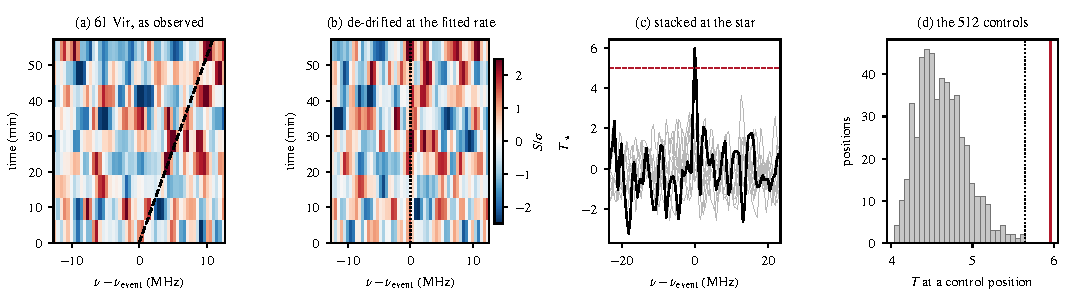
\includegraphics[width=\textwidth]{figures/event_crossings.pdf}
\caption{\textbf{The strongest unattributed crossing of the quality-passing
data, and the control field it leads.} Frequencies are in the star's rest
frame.
\emph{(a)}~The dynamic spectrum at \EvAStar's position around the crossing
at \RqFreqSx\,GHz, observed \EvADate, with the fitted drift of
\EvADrift\,Hz\,s$^{-1}$ as the dashed track. The \EvANInt{} integrations are
binned into \EvANBin{} and plotted in units of each bin's noise. At
\EvAFlux$\pm$\EvAFluxErr\,mJy against \EvARmsInt\,mJy per integration the
carrier is \EvAPerIntSig{} standard deviations in any one of them, and exists
only in the drift-aligned stack of all \EvADwellMin{} minutes on source.
\emph{(b)}~The same rows shifted by that drift, which carries the carrier
\EvADriftChan{} channels of \EvAChanwkHz\,kHz across the
\EvAElapsedMin{} minutes of elapsed time the block spans, not the
\EvADwellMin{} on source.
\emph{(c)}~The de-drifted stack at the star (black) and at the
\RcNRetCtrl{} control positions with retained dynamic spectra (grey), in
units of its own noise; dashed, the trigger. \emph{(d)}~The same statistic at
each of the \NCtrl{} rank-screen control positions: the star (solid) against
the highest control (dotted). The recurrence test for this crossing, and for the second one --
\EvBStar{} at \RqFreqCp\,GHz -- is in Table~\ref{tab:cand}.}
\label{fig:event}
\end{figure*}

\begin{table}
\centering
\caption{\textbf{Can two crossings be one carrier?} Every pair of crossings
toward one star, in two execution blocks, lying within
$\pm\WdHalfKms$\,km\,s$^{-1}$ of each other in the star's frame -- the
half-width of the median spectral window a repeat could be found in -- and
carrying between them two independently fitted drifts and two block epochs
measured from their own data: \TjNPair{} pairs with an unattributed member,
of the \TjNCandPair{} inside that interval. Below the rule is the control, the
\TjNCandAttrTest{} of \TjNCandAttr{} pairs of already attributed crossings for
which a drift and an epoch were both recorded; it is a line that does not
drift, so it shows the test accepting a pair at one frequency and not a
drifting carrier. Stars are
identified by position, so the two archival-tail crossings of \TjDeepStar{}
pair with its catalogued ones. $\Delta\nu$ is the stellar-frame offset and
$\dot\nu_1$, $\dot\nu_2$ the drifts fitted independently in the two blocks
and carried into that frame. A carrier whose drift changes at a constant rate
between the epochs would put the pair at
$\Delta\nu=\frac{1}{2}(\dot\nu_1+\dot\nu_2)\Delta t$; constant
line-of-sight acceleration is the special case $\dot\nu_1=\dot\nu_2$, which
\TjNUneqDrift{} of these pairs fail outright. \emph{Miss} is how
far the pair is from that prediction in units of the drift grid's resolution
carried over $\Delta t$, which is also the resolution the comparison has on
the mean of the two drifts; a dash means it exceeds the window searched, so the
comparison has no power at all. The last column is the verdict under the weaker
criterion of a trajectory whose drift stays inside the searched grid:
\emph{no} where no such trajectory joins the pair, \emph{open} where the pair
is not separable -- neither a confirmation nor an exclusion --
\emph{yes} for the control row. The subscript $\star$ marks the star's
frame, in which the drifts are given; the grid was stepped in the
observatory's, and Table~\ref{tab:edge} gives the rates in it. \EgNPairDriftEdge{} of the rates
printed here, \EgStarDriftHzS\,Hz\,s$^{-1}$ toward \EgStarALosHiStar, is the
outermost trial of its own window's grid: there the search reached the edge
of the interval it covers, so the rate is a lower bound --
\EgStarALosHi\,m\,s$^{-2}$ or more -- and every pair that uses it is marked
\emph{edge} rather than \emph{open}. The exception is the row the criterion
separates, whose verdict uses neither rate: that pair's own offset of
\EgExclOffMHz\,MHz is \EgExclFac{} times the \EgExclReachMHz\,MHz the
ceiling permits over \EgExclDtH\,hours, whatever the two rates are.
Appendix~\ref{sec:edge} establishes the grid's edges and lists every
edge-limited crossing.}
\label{tab:pairs}
\scriptsize
%% GENERATED by pairs_v415.py -- do not hand-edit.
\begin{tabular}{@{}l@{~}l@{\hspace{4pt}}r@{\,}r@{\,}r@{\,}r@{\hspace{3.5pt}}r@{~}l@{}}
\hline
Star & blocks & $\Delta t$ & $\dot\nu_{1\star}$ & $\dot\nu_{2\star}$ & $\Delta\nu$ & miss & one \\
 & & (d) & \multicolumn{2}{c}{(Hz\,s$^{-1}$)} & (MHz) & ($\sigma$) & carrier? \\
\hline
61~Vir & X822/X82f & 3.00 & $+1092$ & $+3221$ & $+755.4$ & 15 & open \\
J1537$-$3319 & X10359/X398 & 123 & $-2000$ & $+2390$ & $+223.5$ & 3.6 & open \\
AU~Mic & X1838/X319 & 310 & $+1440$ & $+2645$ & $-159.0$ & -- & open \\
HD~14055 & X2b2ee/X2c3bb & 0.09 & $-2390$ & $+4216$ & $+825.2$ & 2447 & no \\
 & X24be0/Xd46 & 1.92 & $+1134$ & $-3823$ & $+63.0$ & 41 & open \\
 & X2c3bb/X3835 & 2.00 & $+4216$ & $+1800$ & $-514.6$ & 144 & edge \\
 & X2b2ee/X3835 & 2.09 & $-2390$ & $+1800$ & $+310.6$ & 48 & open \\
 & X3835/Xd526 & 607 & $+1800$ & $-2563$ & $-555.5$ & -- & open \\
 & X2b2ee/Xd526 & 609 & $-2390$ & $-2563$ & $-244.9$ & -- & open \\
 & X3835/X25c5e & 649 & $+1800$ & $+2611$ & $+423.3$ & -- & open \\
 & X2c3bb/X25c5e & 651 & $+4216$ & $+2611$ & $-91.3$ & -- & edge \\
 & X2b2ee/X25c5e & 651 & $-2390$ & $+2611$ & $+733.8$ & -- & open \\
$\beta$~Pic & X3a90/Xa9df & 1.02 & $-1611$ & $-679$ & $+85.5$ & 132 & open \\
\hline
HD~285968 & X108f/X5b4e & 4.99 & $-29$ & $-29$ & $-0.002$ & 0.6 & yes \\
\hline
\end{tabular}

\end{table}

\begin{table}
\centering
\caption{\textbf{The two events}, the crossings whose
stellar statistic exceeds all \NCtrl{} control positions of their own window;
the first of them is Fig.~\ref{fig:event}.
Repeat epochs measured are the blocks at which the predicted stellar-frame
cell was read, the remainder of them coming from the reserved hold-out and the
archival extension.
$T_{\rm pers}$ is what a carrier persisting at the discovery amplitude $S$
would have given there and $T_{\rm rep}$ is what is measured, combining every
repeat epoch by inverse variance at the carried drift: one cell and one
trial, so it may be negative, while the two indented readings beneath it are
maxima and so positive on average whatever is there -- the second of them
the same cell at every trial of the window's own drift grid, which bounds an
error in the carried drift. The nearest block alone
follows, because the combination asks the model of \S\ref{sec:etacrv} of
every block across the whole baseline while the single reading asks it only
of the two observations. The exclusion is the fraction of $S$ still
ruled out at the trigger, $(T_{\rm rep}+5)/T_{\rm pers}$; the displacement
permitted is half a channel in the star's frame. The last row but one is the
chance $\Phi(5T_{\rm pers}/T_\star-5)$ that a carrier at the trigger
amplitude $5S/T_\star$ would have satisfied the criterion, and in brackets the
same at $S$, which is selected as the largest of many cells and biased high.}
\label{tab:cand}
\footnotesize
%% GENERATED by recur_v411.py -- do not hand-edit.
\begin{tabular}{@{}>{\raggedright\arraybackslash}p{0.49\columnwidth}@{~~}r@{~~}r@{}}
\hline
 & 61 Vir & CP$-$72 2713 \\
\hline
Frequency, stellar frame (GHz) & 346.323236 & 344.296455 \\
\quad as delivered, topocentric & 346.313811 & 344.269746 \\
Drift rate (Hz\,s$^{-1}$) & $+3182$ & $-2056$ \\
$T_\star$ & 5.958 & 5.809 \\
Highest control $T$ & 5.65 & 5.68 \\
Fitted amplitude (mJy) & 118.8 $\pm$ 19.9 & 11.3 $\pm$ 2.0 \\
Peak-channel EIRP (W) & $5.1 \times 10^{14}$ & $8.9 \times 10^{14}$ \\
Repeat epochs measured & 3 & 5 \\
\quad of them in the primary census & 3 & 1 \\
\quad census repeats with no retained spectrum & 1 & 0 \\
Nearest covering epoch, separation (h) & $-1.97$ & $+2.05$ \\
\quad covering epochs more than a day away & 2 & 4 \\
Longest baseline (d) & 3 & 2 \\
$T$ expected if persistent, $T_{\rm pers}$ & 9.70 & 6.30 \\
$T$ measured, matched drift, $T_{\rm rep}$ & $+0.39$ & $-0.82$ \\
\quad largest single epoch & $+1.65$ & $+0.96$ \\
\quad maximised over every drift & 2.71 & 3.60 \\
Nearest block alone, $T_{\rm pers}$ & 5.28 & 6.21 \\
\quad $T_{\rm rep}$ & $-0.01$ & $-0.57$ \\
Amplitude still excluded, $(T_{\rm rep}+5)/T_{\rm pers}$ & 0.56 $S$ & 0.66 $S$ \\
\quad from the nearest block alone & 0.95 $S$ & 0.71 $S$ \\
\quad from separated blocks alone & \SpSxFracSep{} $S$ ($n=\SpSxNSep$) & \SpCpFracSep{} $S$ ($n=\SpCpNSep$) \\
\quad over the matched registration tolerance & \SpSxFracTol{} $S$ & \SpCpFracTol{} $S$ \\
Displacement permitted (km\,s$^{-1}$) & $\pm$0.211 & $\pm$0.213 \\
Recovery chance at $5S/T_\star$ (at $S$) & 1.00 (1.00) & 0.66 (0.90) \\
Disposition & not confirmed & not confirmed \\
\hline
\end{tabular}

\end{table}

\begin{table*}
\centering
\caption{\textbf{The threshold crossings of the reserved hold-out}, searched
with the same pipeline and disposed of by the same tests as the
census. $\Delta v_\star$ is the offset from the nearest masked transition in
the star's own frame and $n_{\rm rep}$ the number of covering repeat blocks;
$T_{\rm pers}$ and $T_{\rm rep}$ are as in the crossing ledger. The one
crossing that is present again is a carbon monoxide line. A dagger marks an
offset inside the attribution interval whose species the attribution set
excludes, as in the crossing ledger; such a crossing is reported and not
acted on (Appendix~\ref{app:linemask}).}
\label{tab:holdout}
\scriptsize
%% GENERATED by holdout_v412.py -- do not hand-edit.
\begin{tabular}{@{}l@{~}l@{~}r@{~}r@{~}l@{~}r@{~~}r@{~}r@{~}r@{~}l@{}}
\hline
Star & block & $\nu_{\rm topo}$ (GHz) & $T_\star$ & line & $\Delta v_\star$ & $n_{\rm rep}$ & $T_{\rm pers}$ & $T_{\rm rep}$ & disposition \\
\hline
HD~285968 & Xdaef5a\_Xdd9b & 230.5081 & 8.642 & CO($2$--$1$) & +8.7 & 4 & 11.6 & +6.71 & attributed; present again \\
HD~14055 & X107376c\_X6126 & 330.7123 & 5.513 & $^{13}$CO($3$--$2$) & +112.6 & 30 & 312.0 & +0.56 & unattributed; does not recur \\
TRAPPIST$-$1 & Xd0e450\_X259b & 346.2454 & 5.326 & SO($9_{8}$--$8_{7}$) & \ensuremath{-}306.6 & 5 & 11.1 & \ensuremath{-}0.32 & unattributed; does not recur \\
HD~172555 & X107fa96\_X1300f & 344.6066 & 5.144 & SO($8_{8}$--$7_{7}$) & +251.3 & -- & -- & -- & unattributed; no repeat coverage \\
HD~285968 & Xdb4b9a\_Xa7c & 229.9129 & 5.106 & CO($2$--$1$) & \ensuremath{-}768.0 & 4 & 11.2 & +0.21 & unattributed; does not recur \\
HR~1010 & Xc6b674\_X23f2 & 346.2301 & 5.044 & SO($9_{8}$--$8_{7}$) & \ensuremath{-}238.7 & 7 & 25.9 & \ensuremath{-}0.80 & unattributed; does not recur \\
HD~10647 & Xff99e1\_X9cdf & 345.7059 & 5.017 & SO($2_{3}$--$2_{1}$) & +37.1$^{\dagger}$ & 13 & 142.1 & \ensuremath{-}0.93 & unattributed; does not recur \\
HD~170773 & Xff294f\_X1fb & 345.5597 & 5.001 & SO($2_{3}$--$2_{1}$) & \ensuremath{-}113.8 & 4 & 59.3 & +1.45 & unattributed; does not recur \\
\hline
\end{tabular}

\end{table*}

%% tab:ledger MOVED to Appendix D (sections/app_J_falsealarm.tex): a
%% full-width 56-row table* worth 0.72 pp of the main text.  Sec. 5.3 and
%% Sec. 5.6 carry the counts and cite it.



%% fig:chain MOVED to sections/04_method.tex, Sec. 4.2, where it is first
%% cited (referee 2, minor 3).  Sec. 5 cites it at the crossing census.
